\documentclass[twoside]{book}

% Packages required by doxygen
\usepackage{fixltx2e}
\usepackage{calc}
\usepackage{doxygen}
\usepackage[export]{adjustbox} % also loads graphicx
\usepackage{graphicx}
\usepackage[utf8]{inputenc}
\usepackage{makeidx}
\usepackage{multicol}
\usepackage{multirow}
\PassOptionsToPackage{warn}{textcomp}
\usepackage{textcomp}
\usepackage[nointegrals]{wasysym}
\usepackage[table]{xcolor}

% Font selection
\usepackage[T1]{fontenc}
\usepackage[scaled=.90]{helvet}
\usepackage{courier}
\usepackage{amssymb}
\usepackage{sectsty}
\renewcommand{\familydefault}{\sfdefault}
\allsectionsfont{%
  \fontseries{bc}\selectfont%
  \color{darkgray}%
}
\renewcommand{\DoxyLabelFont}{%
  \fontseries{bc}\selectfont%
  \color{darkgray}%
}
\newcommand{\+}{\discretionary{\mbox{\scriptsize$\hookleftarrow$}}{}{}}

% Page & text layout
\usepackage{geometry}
\geometry{%
  a4paper,%
  top=2.5cm,%
  bottom=2.5cm,%
  left=2.5cm,%
  right=2.5cm%
}
\tolerance=750
\hfuzz=15pt
\hbadness=750
\setlength{\emergencystretch}{15pt}
\setlength{\parindent}{0cm}
\setlength{\parskip}{3ex plus 2ex minus 2ex}
\makeatletter
\renewcommand{\paragraph}{%
  \@startsection{paragraph}{4}{0ex}{-1.0ex}{1.0ex}{%
    \normalfont\normalsize\bfseries\SS@parafont%
  }%
}
\renewcommand{\subparagraph}{%
  \@startsection{subparagraph}{5}{0ex}{-1.0ex}{1.0ex}{%
    \normalfont\normalsize\bfseries\SS@subparafont%
  }%
}
\makeatother

% Headers & footers
\usepackage{fancyhdr}
\pagestyle{fancyplain}
\fancyhead[LE]{\fancyplain{}{\bfseries\thepage}}
\fancyhead[CE]{\fancyplain{}{}}
\fancyhead[RE]{\fancyplain{}{\bfseries\leftmark}}
\fancyhead[LO]{\fancyplain{}{\bfseries\rightmark}}
\fancyhead[CO]{\fancyplain{}{}}
\fancyhead[RO]{\fancyplain{}{\bfseries\thepage}}
\fancyfoot[LE]{\fancyplain{}{}}
\fancyfoot[CE]{\fancyplain{}{}}
\fancyfoot[RE]{\fancyplain{}{\bfseries\scriptsize Generated by Doxygen }}
\fancyfoot[LO]{\fancyplain{}{\bfseries\scriptsize Generated by Doxygen }}
\fancyfoot[CO]{\fancyplain{}{}}
\fancyfoot[RO]{\fancyplain{}{}}
\renewcommand{\footrulewidth}{0.4pt}
\renewcommand{\chaptermark}[1]{%
  \markboth{#1}{}%
}
\renewcommand{\sectionmark}[1]{%
  \markright{\thesection\ #1}%
}

% Indices & bibliography
\usepackage{natbib}
\usepackage[titles]{tocloft}
\setcounter{tocdepth}{3}
\setcounter{secnumdepth}{5}
\makeindex

% Hyperlinks (required, but should be loaded last)
\usepackage{ifpdf}
\ifpdf
  \usepackage[pdftex,pagebackref=true]{hyperref}
\else
  \usepackage[ps2pdf,pagebackref=true]{hyperref}
\fi
\hypersetup{%
  colorlinks=true,%
  linkcolor=blue,%
  citecolor=blue,%
  unicode%
}

% Custom commands
\newcommand{\clearemptydoublepage}{%
  \newpage{\pagestyle{empty}\cleardoublepage}%
}

\usepackage{caption}
\captionsetup{labelsep=space,justification=centering,font={bf},singlelinecheck=off,skip=4pt,position=top}

%===== C O N T E N T S =====

\begin{document}

% Titlepage & ToC
\hypersetup{pageanchor=false,
             bookmarksnumbered=true,
             pdfencoding=unicode
            }
\pagenumbering{alph}
\begin{titlepage}
\vspace*{7cm}
\begin{center}%
{\Large Text\+Box Library }\\
\vspace*{1cm}
{\large Generated by Doxygen 1.8.13}\\
\end{center}
\end{titlepage}
\clearemptydoublepage
\pagenumbering{roman}
\tableofcontents
\clearemptydoublepage
\pagenumbering{arabic}
\hypersetup{pageanchor=true}

%--- Begin generated contents ---
\chapter{Overview}
\label{index}\hypertarget{index}{}Text\+Box Library or \textquotesingle{}libtb\textquotesingle{} is a C++ A\+PI used to interface with Text\+Boxes. Visit the \href{https://codrod.github.io/gtb/index.html}{\tt gtb} repository to learn more about Text\+Boxes. 
\chapter{Text\+Box Library}
\label{a00057}
\Hypertarget{a00057}
\subsubsection*{Overview}

Text\+Box Library or \textquotesingle{}libtb\textquotesingle{} is a C++ A\+PI used to interface with Text\+Boxes. Visit the \href{https://codrod.github.io/gtb/index.html}{\tt gtb} repository to learn more about Text\+Boxes.

\subsubsection*{Documentation}

Documentation is generated by Doxygen and hosted on \href{https://codrod.github.io/libtb/index.html}{\tt Git\+Hub Pages}.

\subsubsection*{Build Instructions}


\begin{DoxyItemize}
\item make
\item make docs
\end{DoxyItemize}

\subsubsection*{Development Status}


\begin{DoxyItemize}
\item cursor control/positioning -\/ completed
\item insert output -\/ completed
\item clear output -\/ completed
\item scroll output -\/ completed
\item edit line -\/ completed
\item embedded images -\/ in progress
\item event driven key binding -\/ not started
\end{DoxyItemize}

\subsubsection*{Development Plan}


\begin{DoxyEnumerate}
\item Add unit testing
\item Improve documentation
\item Complete current features
\item Windows port 
\end{DoxyEnumerate}
\chapter{Hierarchical Index}
\section{Class Hierarchy}
This inheritance list is sorted roughly, but not completely, alphabetically\+:\begin{DoxyCompactList}
\item \contentsline{section}{Text\+Box\+:\+:Box}{\pageref{a00032}}{}
\item \contentsline{section}{Text\+Box\+:\+:coord}{\pageref{a00016}}{}
\item \contentsline{section}{Text\+Box\+:\+:Input\+Pipe}{\pageref{a00044}}{}
\item istream\begin{DoxyCompactList}
\item \contentsline{section}{Text\+Box\+:\+:istream}{\pageref{a00028}}{}
\end{DoxyCompactList}
\item \contentsline{section}{Text\+Box\+:\+:Mutex}{\pageref{a00036}}{}
\item ostream\begin{DoxyCompactList}
\item \contentsline{section}{Text\+Box\+:\+:ostream}{\pageref{a00024}}{}
\end{DoxyCompactList}
\item \contentsline{section}{Text\+Box\+:\+:Output\+Pipe}{\pageref{a00040}}{}
\item vector\begin{DoxyCompactList}
\item \contentsline{section}{Text\+Box\+:\+:Sequence}{\pageref{a00020}}{}
\end{DoxyCompactList}
\end{DoxyCompactList}

\chapter{Class Index}
\section{Class List}
Here are the classes, structs, unions and interfaces with brief descriptions\+:\begin{DoxyCompactList}
\item\contentsline{section}{\hyperlink{a00032}{Text\+Box\+::\+Box} }{\pageref{a00032}}{}
\item\contentsline{section}{\hyperlink{a00016}{Text\+Box\+::coord} }{\pageref{a00016}}{}
\item\contentsline{section}{\hyperlink{a00044}{Text\+Box\+::\+Input\+Pipe} }{\pageref{a00044}}{}
\item\contentsline{section}{\hyperlink{a00028}{Text\+Box\+::istream} }{\pageref{a00028}}{}
\item\contentsline{section}{\hyperlink{a00036}{Text\+Box\+::\+Mutex} }{\pageref{a00036}}{}
\item\contentsline{section}{\hyperlink{a00024}{Text\+Box\+::ostream} }{\pageref{a00024}}{}
\item\contentsline{section}{\hyperlink{a00040}{Text\+Box\+::\+Output\+Pipe} }{\pageref{a00040}}{}
\item\contentsline{section}{\hyperlink{a00020}{Text\+Box\+::\+Sequence} }{\pageref{a00020}}{}
\end{DoxyCompactList}

\chapter{File Index}
\section{File List}
Here is a list of all documented files with brief descriptions\+:\begin{DoxyCompactList}
\item\contentsline{section}{\hyperlink{a00005}{textbox.\+h} \\*Header file for libtb }{\pageref{a00005}}{}
\item\contentsline{section}{\hyperlink{a00008}{textbox\+\_\+posix.\+h} \\*P\+O\+S\+IX middleware for libtb }{\pageref{a00008}}{}
\end{DoxyCompactList}

\chapter{Class Documentation}
\hypertarget{a00032}{}\section{Text\+Box\+:\+:Box Class Reference}
\label{a00032}\index{Text\+Box\+::\+Box@{Text\+Box\+::\+Box}}


Collaboration diagram for Text\+Box\+:\+:Box\+:\nopagebreak
\begin{figure}[H]
\begin{center}
\leavevmode
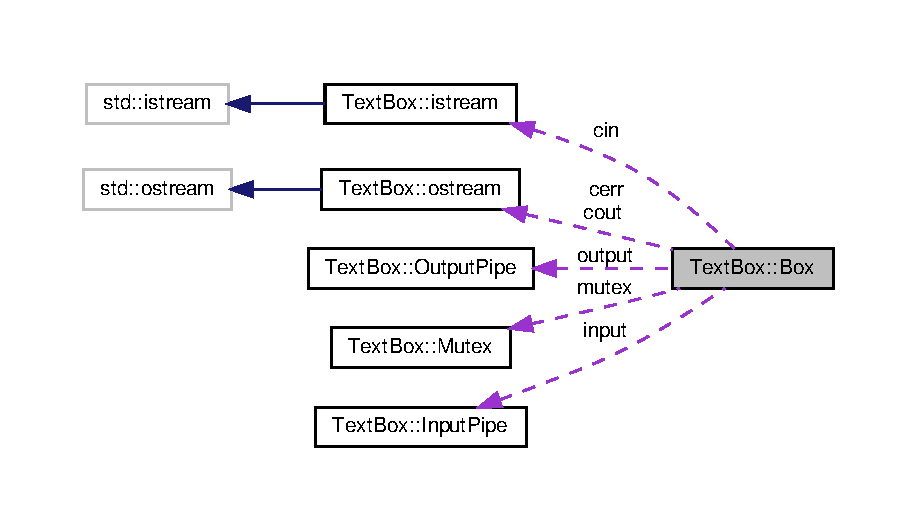
\includegraphics[width=350pt]{a00030}
\end{center}
\end{figure}
\subsection*{Public Member Functions}
\begin{DoxyCompactItemize}
\item 
\mbox{\Hypertarget{a00032_ad1ff097a7299048f3efbca46f6c8844d}\label{a00032_ad1ff097a7299048f3efbca46f6c8844d}} 
\hyperlink{a00032}{Box} \& {\bfseries lock} ()
\item 
\mbox{\Hypertarget{a00032_a4f79c74df9a31294b05f92a131fdddd0}\label{a00032_a4f79c74df9a31294b05f92a131fdddd0}} 
\hyperlink{a00032}{Box} \& {\bfseries unlock} ()
\item 
\mbox{\Hypertarget{a00032_a9d5caf4fb5c26fbed60a4686bb81d291}\label{a00032_a9d5caf4fb5c26fbed60a4686bb81d291}} 
std\+::string {\bfseries get\+D\+CS} ()
\item 
\mbox{\Hypertarget{a00032_a9033777e3b7f666c61a96412e7312af4}\label{a00032_a9033777e3b7f666c61a96412e7312af4}} 
\hyperlink{a00032}{Box} \& {\bfseries put\+D\+CS} (std\+::string seq)
\item 
\mbox{\Hypertarget{a00032_a6c56ae4253031c1ed9a5f6ca558769b0}\label{a00032_a6c56ae4253031c1ed9a5f6ca558769b0}} 
\hyperlink{a00020}{Sequence} {\bfseries send\+D\+CS} (std\+::string seqstr, std\+::string err, int retsiz)
\end{DoxyCompactItemize}
\subsection*{Public Attributes}
\begin{DoxyCompactItemize}
\item 
\mbox{\Hypertarget{a00032_ac21d0f2a85262aa622fb31bef2370139}\label{a00032_ac21d0f2a85262aa622fb31bef2370139}} 
\hyperlink{a00036}{Mutex} $\ast$ {\bfseries mutex}
\item 
\mbox{\Hypertarget{a00032_a0b732f6f64029291a7f756f8bcfc85b6}\label{a00032_a0b732f6f64029291a7f756f8bcfc85b6}} 
\hyperlink{a00040}{Output\+Pipe} $\ast$ {\bfseries output}
\item 
\mbox{\Hypertarget{a00032_aa1cea72263f267f73fb61ec4d807fd68}\label{a00032_aa1cea72263f267f73fb61ec4d807fd68}} 
\hyperlink{a00044}{Input\+Pipe} $\ast$ {\bfseries input}
\item 
\mbox{\Hypertarget{a00032_aa21ac76f8ec37149bc6349ef7a111ec1}\label{a00032_aa21ac76f8ec37149bc6349ef7a111ec1}} 
\hyperlink{a00028}{istream} {\bfseries cin}
\item 
\mbox{\Hypertarget{a00032_a6593b812c31f434952d5f1e641b35ce0}\label{a00032_a6593b812c31f434952d5f1e641b35ce0}} 
\hyperlink{a00024}{ostream} {\bfseries cout}
\item 
\mbox{\Hypertarget{a00032_a9c4b838413838baf7c20c01f2a8ca373}\label{a00032_a9c4b838413838baf7c20c01f2a8ca373}} 
\hyperlink{a00024}{ostream} {\bfseries cerr}
\end{DoxyCompactItemize}


The documentation for this class was generated from the following file\+:\begin{DoxyCompactItemize}
\item 
\hyperlink{a00005}{textbox.\+h}\end{DoxyCompactItemize}

\hypertarget{a00016}{}\section{Text\+Box\+:\+:coord Class Reference}
\label{a00016}\index{Text\+Box\+::coord@{Text\+Box\+::coord}}
\subsection*{Public Member Functions}
\begin{DoxyCompactItemize}
\item 
\mbox{\Hypertarget{a00016_a45f1b7e91f95b4a3eecf911b7a1d9a72}\label{a00016_a45f1b7e91f95b4a3eecf911b7a1d9a72}} 
{\bfseries coord} (long long int x, long long int y)
\end{DoxyCompactItemize}
\subsection*{Public Attributes}
\begin{DoxyCompactItemize}
\item 
\mbox{\Hypertarget{a00016_afbe957866d778f4be672a5a0c91058e9}\label{a00016_afbe957866d778f4be672a5a0c91058e9}} 
long long int {\bfseries x}
\item 
\mbox{\Hypertarget{a00016_a72c8755a6bb77c078293dc1b2101f333}\label{a00016_a72c8755a6bb77c078293dc1b2101f333}} 
long long int {\bfseries y}
\end{DoxyCompactItemize}


The documentation for this class was generated from the following file\+:\begin{DoxyCompactItemize}
\item 
\hyperlink{a00005}{textbox.\+h}\end{DoxyCompactItemize}

\hypertarget{a00044}{}\section{Text\+Box\+:\+:Input\+Pipe Class Reference}
\label{a00044}\index{Text\+Box\+::\+Input\+Pipe@{Text\+Box\+::\+Input\+Pipe}}
\subsection*{Public Member Functions}
\begin{DoxyCompactItemize}
\item 
\mbox{\Hypertarget{a00044_a8db53b6915fad69a7415a4cb2b314e71}\label{a00044_a8db53b6915fad69a7415a4cb2b314e71}} 
\hyperlink{a00044}{Input\+Pipe} \& {\bfseries read} (char $\ast$str, std\+::streamsize)
\end{DoxyCompactItemize}


The documentation for this class was generated from the following file\+:\begin{DoxyCompactItemize}
\item 
\hyperlink{a00008}{textbox\+\_\+posix.\+h}\end{DoxyCompactItemize}

\hypertarget{a00028}{}\section{Text\+Box\+:\+:istream Class Reference}
\label{a00028}\index{Text\+Box\+::istream@{Text\+Box\+::istream}}


Inheritance diagram for Text\+Box\+:\+:istream\+:\nopagebreak
\begin{figure}[H]
\begin{center}
\leavevmode
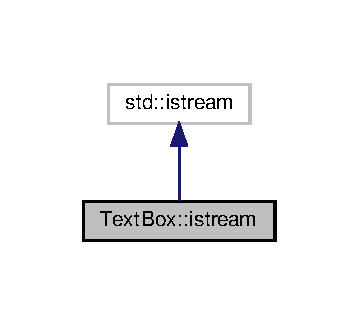
\includegraphics[width=172pt]{a00027}
\end{center}
\end{figure}


Collaboration diagram for Text\+Box\+:\+:istream\+:\nopagebreak
\begin{figure}[H]
\begin{center}
\leavevmode
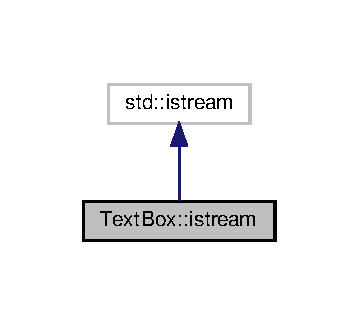
\includegraphics[width=172pt]{a00026}
\end{center}
\end{figure}
\subsection*{Public Member Functions}
\begin{DoxyCompactItemize}
\item 
\mbox{\Hypertarget{a00028_ae5080239d7ee3af9b44560f93ae27bb2}\label{a00028_ae5080239d7ee3af9b44560f93ae27bb2}} 
{\bfseries istream} (\hyperlink{a00032}{Box} $\ast$box)
\item 
\mbox{\Hypertarget{a00028_ad447d78602bdb69cd6506de8743cc014}\label{a00028_ad447d78602bdb69cd6506de8743cc014}} 
\hyperlink{a00028}{istream} \& {\bfseries move} (\hyperlink{a00016}{coord} pos)
\item 
\mbox{\Hypertarget{a00028_ab7b3c484d049f7827462a35cca79c62c}\label{a00028_ab7b3c484d049f7827462a35cca79c62c}} 
\hyperlink{a00016}{coord} {\bfseries find} ()
\item 
\mbox{\Hypertarget{a00028_af72da4d27ba8c504d9ee2e6ceab90056}\label{a00028_af72da4d27ba8c504d9ee2e6ceab90056}} 
\hyperlink{a00028}{istream} \& {\bfseries editline} (char $\ast$str, std\+::streamsize siz)
\end{DoxyCompactItemize}


The documentation for this class was generated from the following file\+:\begin{DoxyCompactItemize}
\item 
\hyperlink{a00005}{textbox.\+h}\end{DoxyCompactItemize}

\hypertarget{a00036}{}\section{Text\+Box\+:\+:Mutex Class Reference}
\label{a00036}\index{Text\+Box\+::\+Mutex@{Text\+Box\+::\+Mutex}}
\subsection*{Public Member Functions}
\begin{DoxyCompactItemize}
\item 
\mbox{\Hypertarget{a00036_acf898d827d4c3c79e0f7ce18ae594814}\label{a00036_acf898d827d4c3c79e0f7ce18ae594814}} 
\hyperlink{a00036}{Mutex} \& {\bfseries lock} ()
\item 
\mbox{\Hypertarget{a00036_a4789aa2933baf457108b9c1f4b9f6c4f}\label{a00036_a4789aa2933baf457108b9c1f4b9f6c4f}} 
\hyperlink{a00036}{Mutex} \& {\bfseries unlock} ()
\end{DoxyCompactItemize}


The documentation for this class was generated from the following file\+:\begin{DoxyCompactItemize}
\item 
\hyperlink{a00008}{textbox\+\_\+posix.\+h}\end{DoxyCompactItemize}

\hypertarget{a00024}{}\section{Text\+Box\+:\+:ostream Class Reference}
\label{a00024}\index{Text\+Box\+::ostream@{Text\+Box\+::ostream}}


Inheritance diagram for Text\+Box\+:\+:ostream\+:\nopagebreak
\begin{figure}[H]
\begin{center}
\leavevmode
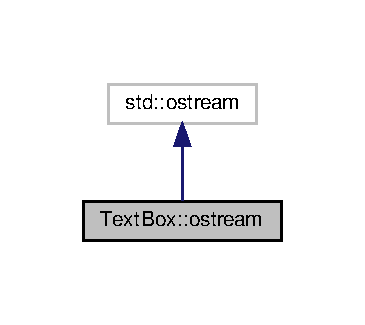
\includegraphics[width=175pt]{a00023}
\end{center}
\end{figure}


Collaboration diagram for Text\+Box\+:\+:ostream\+:\nopagebreak
\begin{figure}[H]
\begin{center}
\leavevmode
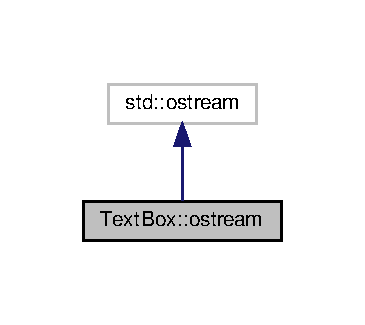
\includegraphics[width=175pt]{a00022}
\end{center}
\end{figure}
\subsection*{Public Member Functions}
\begin{DoxyCompactItemize}
\item 
\mbox{\Hypertarget{a00024_a7731093fa8055859dbd787daccf05487}\label{a00024_a7731093fa8055859dbd787daccf05487}} 
{\bfseries ostream} (\hyperlink{a00032}{Box} $\ast$box)
\item 
\mbox{\Hypertarget{a00024_a5d54f321f1c93a532187cecd7066abfb}\label{a00024_a5d54f321f1c93a532187cecd7066abfb}} 
\hyperlink{a00024}{ostream} \& {\bfseries move} (\hyperlink{a00016}{coord} pos)
\item 
\mbox{\Hypertarget{a00024_a668803d866c61762e43afaebbaab7e23}\label{a00024_a668803d866c61762e43afaebbaab7e23}} 
\hyperlink{a00016}{coord} {\bfseries find} ()
\item 
\mbox{\Hypertarget{a00024_a2c464c6349d5251b3af55a60175a66ad}\label{a00024_a2c464c6349d5251b3af55a60175a66ad}} 
\hyperlink{a00024}{ostream} \& {\bfseries scroll} (\hyperlink{a00016}{coord} pos)
\item 
\mbox{\Hypertarget{a00024_a57afd191cfe61c5a5520cfbf3c67c442}\label{a00024_a57afd191cfe61c5a5520cfbf3c67c442}} 
\hyperlink{a00024}{ostream} \& {\bfseries clear} (\hyperlink{a00016}{coord} start, \hyperlink{a00016}{coord} finish)
\item 
\mbox{\Hypertarget{a00024_aa8c666d1e8cca923e3dbe8d97618dbc3}\label{a00024_aa8c666d1e8cca923e3dbe8d97618dbc3}} 
\hyperlink{a00024}{ostream} \& {\bfseries clear} ()
\item 
\mbox{\Hypertarget{a00024_a322785bda06f0ec90877de7c06f8b2b4}\label{a00024_a322785bda06f0ec90877de7c06f8b2b4}} 
\hyperlink{a00024}{ostream} \& {\bfseries write} (const char $\ast$str, std\+::streamsize siz)
\item 
\mbox{\Hypertarget{a00024_a2c35e6b1045c1b49167d64b301375774}\label{a00024_a2c35e6b1045c1b49167d64b301375774}} 
\hyperlink{a00024}{ostream} \& {\bfseries write} (const char $\ast$str)
\item 
\mbox{\Hypertarget{a00024_a559bcf10a372c9b21752150db3f4636d}\label{a00024_a559bcf10a372c9b21752150db3f4636d}} 
\hyperlink{a00024}{ostream} \& {\bfseries put} (char c)
\item 
\mbox{\Hypertarget{a00024_a3bf0d2b4a90765422fbdf7d05dd4a3d4}\label{a00024_a3bf0d2b4a90765422fbdf7d05dd4a3d4}} 
\hyperlink{a00024}{ostream} \& {\bfseries insert} (const char $\ast$str, std\+::streamsize siz)
\item 
\mbox{\Hypertarget{a00024_a0501fcaeaa1306aa12de21f9ca056270}\label{a00024_a0501fcaeaa1306aa12de21f9ca056270}} 
\hyperlink{a00024}{ostream} \& {\bfseries insert} (const char $\ast$str)
\item 
\mbox{\Hypertarget{a00024_a98957e4cc91144fbbc169322fe7dddfa}\label{a00024_a98957e4cc91144fbbc169322fe7dddfa}} 
\hyperlink{a00024}{ostream} \& {\bfseries insert} (char c)
\end{DoxyCompactItemize}


The documentation for this class was generated from the following file\+:\begin{DoxyCompactItemize}
\item 
\hyperlink{a00005}{textbox.\+h}\end{DoxyCompactItemize}

\hypertarget{a00040}{}\section{Text\+Box\+:\+:Output\+Pipe Class Reference}
\label{a00040}\index{Text\+Box\+::\+Output\+Pipe@{Text\+Box\+::\+Output\+Pipe}}
\subsection*{Public Member Functions}
\begin{DoxyCompactItemize}
\item 
\mbox{\Hypertarget{a00040_a45dbdf8eafaa645b77dc9bbad21a8ad3}\label{a00040_a45dbdf8eafaa645b77dc9bbad21a8ad3}} 
\hyperlink{a00040}{Output\+Pipe} \& {\bfseries write} (const char $\ast$str, std\+::streamsize)
\end{DoxyCompactItemize}


The documentation for this class was generated from the following file\+:\begin{DoxyCompactItemize}
\item 
\hyperlink{a00008}{textbox\+\_\+posix.\+h}\end{DoxyCompactItemize}

\hypertarget{a00020}{}\section{Text\+Box\+:\+:Sequence Class Reference}
\label{a00020}\index{Text\+Box\+::\+Sequence@{Text\+Box\+::\+Sequence}}


Inheritance diagram for Text\+Box\+:\+:Sequence\+:\nopagebreak
\begin{figure}[H]
\begin{center}
\leavevmode
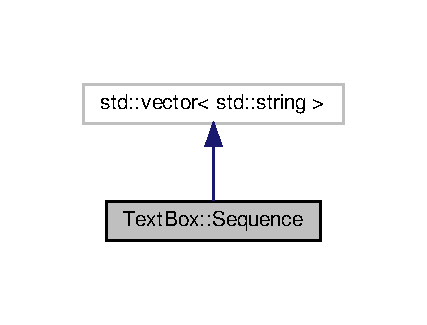
\includegraphics[width=205pt]{a00019}
\end{center}
\end{figure}


Collaboration diagram for Text\+Box\+:\+:Sequence\+:\nopagebreak
\begin{figure}[H]
\begin{center}
\leavevmode
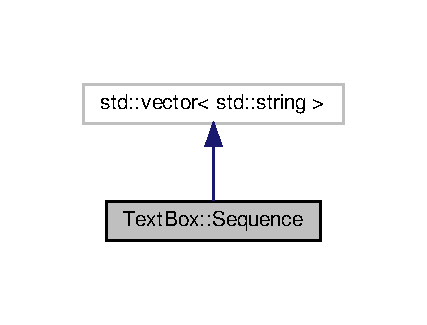
\includegraphics[width=205pt]{a00018}
\end{center}
\end{figure}
\subsection*{Public Member Functions}
\begin{DoxyCompactItemize}
\item 
\mbox{\Hypertarget{a00020_a4577eae876f688f54023ad05dc425e9f}\label{a00020_a4577eae876f688f54023ad05dc425e9f}} 
{\bfseries Sequence} (std\+::string seq)
\item 
\mbox{\Hypertarget{a00020_a492e931d8cc0fc9c43af02ae915c313f}\label{a00020_a492e931d8cc0fc9c43af02ae915c313f}} 
\hyperlink{a00020}{Sequence} \& {\bfseries parse} (std\+::string seq)
\end{DoxyCompactItemize}


The documentation for this class was generated from the following file\+:\begin{DoxyCompactItemize}
\item 
\hyperlink{a00005}{textbox.\+h}\end{DoxyCompactItemize}

\chapter{File Documentation}
\hypertarget{a00005}{}\section{textbox.\+h File Reference}
\label{a00005}\index{textbox.\+h@{textbox.\+h}}


Header file for libtb.  


{\ttfamily \#include $<$stdlib.\+h$>$}\newline
{\ttfamily \#include $<$errno.\+h$>$}\newline
{\ttfamily \#include $<$string.\+h$>$}\newline
{\ttfamily \#include $<$iostream$>$}\newline
{\ttfamily \#include $<$string$>$}\newline
{\ttfamily \#include $<$vector$>$}\newline
{\ttfamily \#include \char`\"{}textbox\+\_\+posix.\+h\char`\"{}}\newline
Include dependency graph for textbox.\+h\+:\nopagebreak
\begin{figure}[H]
\begin{center}
\leavevmode
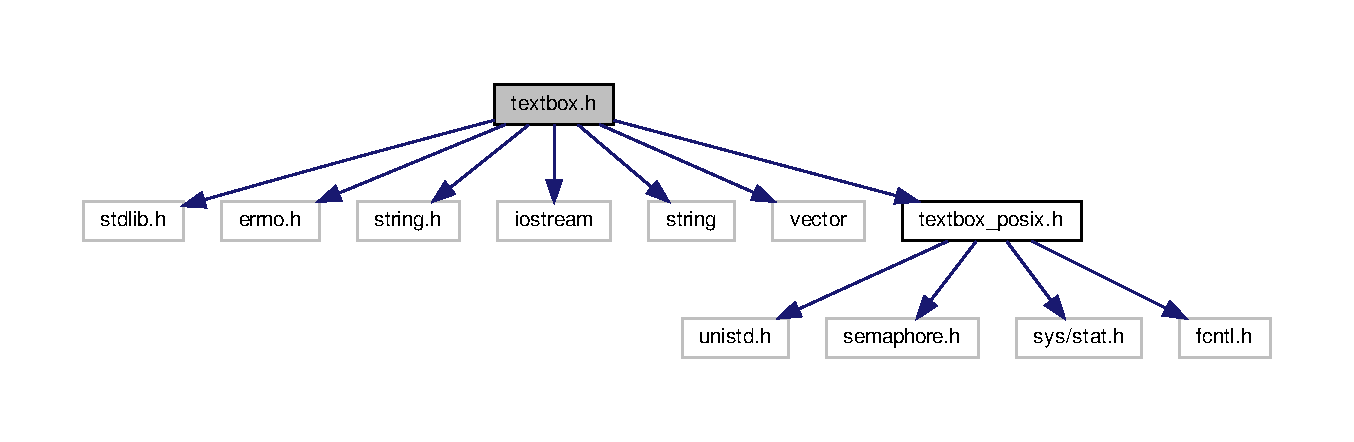
\includegraphics[width=350pt]{a00006}
\end{center}
\end{figure}
\subsection*{Classes}
\begin{DoxyCompactItemize}
\item 
class \hyperlink{a00016}{Text\+Box\+::coord}
\item 
class \hyperlink{a00020}{Text\+Box\+::\+Sequence}
\item 
class \hyperlink{a00024}{Text\+Box\+::ostream}
\item 
class \hyperlink{a00028}{Text\+Box\+::istream}
\item 
class \hyperlink{a00032}{Text\+Box\+::\+Box}
\end{DoxyCompactItemize}
\subsection*{Macros}
\begin{DoxyCompactItemize}
\item 
\mbox{\Hypertarget{a00005_adad9d59e5ec353f6ba40e43478e4946b}\label{a00005_adad9d59e5ec353f6ba40e43478e4946b}} 
\#define {\bfseries T\+E\+X\+T\+B\+O\+X\+\_\+\+V\+E\+R\+S\+I\+ON}~1000000L
\end{DoxyCompactItemize}
\subsection*{Functions}
\begin{DoxyCompactItemize}
\item 
\mbox{\Hypertarget{a00005_a605ed7f7bc6f03b74f770ed27fa9dfa4}\label{a00005_a605ed7f7bc6f03b74f770ed27fa9dfa4}} 
void {\bfseries Text\+Box\+::move\+\_\+cursor} (coord pos)
\end{DoxyCompactItemize}
\subsection*{Variables}
\begin{DoxyCompactItemize}
\item 
\mbox{\Hypertarget{a00005_a5f4c446b39ffcbdbf05f62a3b64795ab}\label{a00005_a5f4c446b39ffcbdbf05f62a3b64795ab}} 
const char {\bfseries Text\+Box\+::\+D\+C1} = \textquotesingle{}\textbackslash{}021\textquotesingle{}
\item 
\mbox{\Hypertarget{a00005_a9d3b75312942d8a8211662bdeaeab239}\label{a00005_a9d3b75312942d8a8211662bdeaeab239}} 
const char {\bfseries Text\+Box\+::\+D\+C2} = \textquotesingle{}\textbackslash{}022\textquotesingle{}
\item 
\mbox{\Hypertarget{a00005_ad81c1964815fe79f9d409a4fa90b8b8c}\label{a00005_ad81c1964815fe79f9d409a4fa90b8b8c}} 
const char {\bfseries Text\+Box\+::\+D\+C3} = \textquotesingle{}\textbackslash{}023\textquotesingle{}
\item 
\mbox{\Hypertarget{a00005_a87aff3a50d54af71a3398935d12a5ed0}\label{a00005_a87aff3a50d54af71a3398935d12a5ed0}} 
\hyperlink{a00032}{Text\+Box\+::\+Box} {\bfseries tb\+::box}
\item 
\mbox{\Hypertarget{a00005_ab5c1751ed3f34d419757e2b6e1d8be55}\label{a00005_ab5c1751ed3f34d419757e2b6e1d8be55}} 
\hyperlink{a00028}{Text\+Box\+::istream} {\bfseries tb\+::cin}
\item 
\mbox{\Hypertarget{a00005_a5e1cc9080f68cbca6e8732e3c1d243e9}\label{a00005_a5e1cc9080f68cbca6e8732e3c1d243e9}} 
\hyperlink{a00024}{Text\+Box\+::ostream} {\bfseries tb\+::cout}
\item 
\mbox{\Hypertarget{a00005_aa114f595f34c913d74da26530dc71494}\label{a00005_aa114f595f34c913d74da26530dc71494}} 
\hyperlink{a00024}{Text\+Box\+::ostream} {\bfseries tb\+::cerr}
\end{DoxyCompactItemize}


\subsection{Detailed Description}
Header file for libtb. 


\hypertarget{a00008}{}\section{textbox\+\_\+posix.\+h File Reference}
\label{a00008}\index{textbox\+\_\+posix.\+h@{textbox\+\_\+posix.\+h}}


P\+O\+S\+IX middleware for libtb.  


{\ttfamily \#include $<$unistd.\+h$>$}\newline
{\ttfamily \#include $<$semaphore.\+h$>$}\newline
{\ttfamily \#include $<$sys/stat.\+h$>$}\newline
{\ttfamily \#include $<$fcntl.\+h$>$}\newline
Include dependency graph for textbox\+\_\+posix.\+h\+:\nopagebreak
\begin{figure}[H]
\begin{center}
\leavevmode
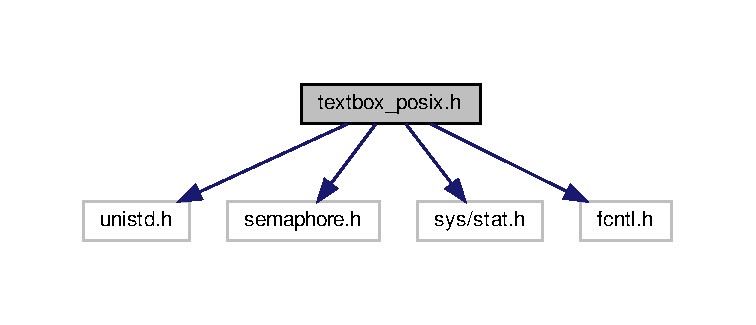
\includegraphics[width=350pt]{a00009}
\end{center}
\end{figure}
This graph shows which files directly or indirectly include this file\+:\nopagebreak
\begin{figure}[H]
\begin{center}
\leavevmode
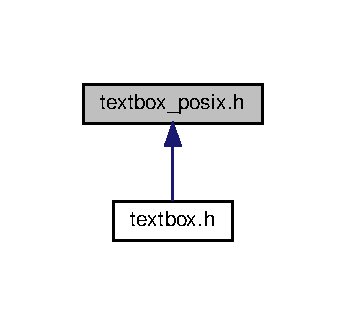
\includegraphics[width=166pt]{a00010}
\end{center}
\end{figure}
\subsection*{Classes}
\begin{DoxyCompactItemize}
\item 
class \hyperlink{a00036}{Text\+Box\+::\+Mutex}
\item 
class \hyperlink{a00040}{Text\+Box\+::\+Output\+Pipe}
\item 
class \hyperlink{a00044}{Text\+Box\+::\+Input\+Pipe}
\end{DoxyCompactItemize}
\subsection*{Macros}
\begin{DoxyCompactItemize}
\item 
\mbox{\Hypertarget{a00008_ad98b2c7915913a840ba875c845dfa070}\label{a00008_ad98b2c7915913a840ba875c845dfa070}} 
\#define {\bfseries T\+E\+X\+T\+B\+O\+X\+\_\+\+P\+O\+S\+I\+X\+\_\+\+V\+ER}~1000000L
\end{DoxyCompactItemize}
\subsection*{Functions}
\begin{DoxyCompactItemize}
\item 
\mbox{\Hypertarget{a00008_aecf0f98513dc0747679b055932e56968}\label{a00008_aecf0f98513dc0747679b055932e56968}} 
char $\ast$ {\bfseries Text\+Box\+::\+Get\+Env} (const char $\ast$name)
\end{DoxyCompactItemize}


\subsection{Detailed Description}
P\+O\+S\+IX middleware for libtb. 


%--- End generated contents ---

% Index
\backmatter
\newpage
\phantomsection
\clearemptydoublepage
\addcontentsline{toc}{chapter}{Index}
\printindex

\end{document}
